% --------------------
  \chapter{Diseño}
% --------------------
\label{C:desarrollo}

En la presente sección se desarrolla el diseño la aplicación y los componentes necesarios para que funcione de forma adecuada. Es necesario establecer que para poder diseñar la aplicación se distribuyen las funciones de la misma por medio de distintos componentes. Asegurando así que se tenga pruebas de que cada componente tiene un funcionamiento correcto por separado como en conjunto. En la figura (\ref{appdiagram}), se puede ver como se distribuyó el diseño de la aplicación.
\begin{figure}[h!]
    \centering
    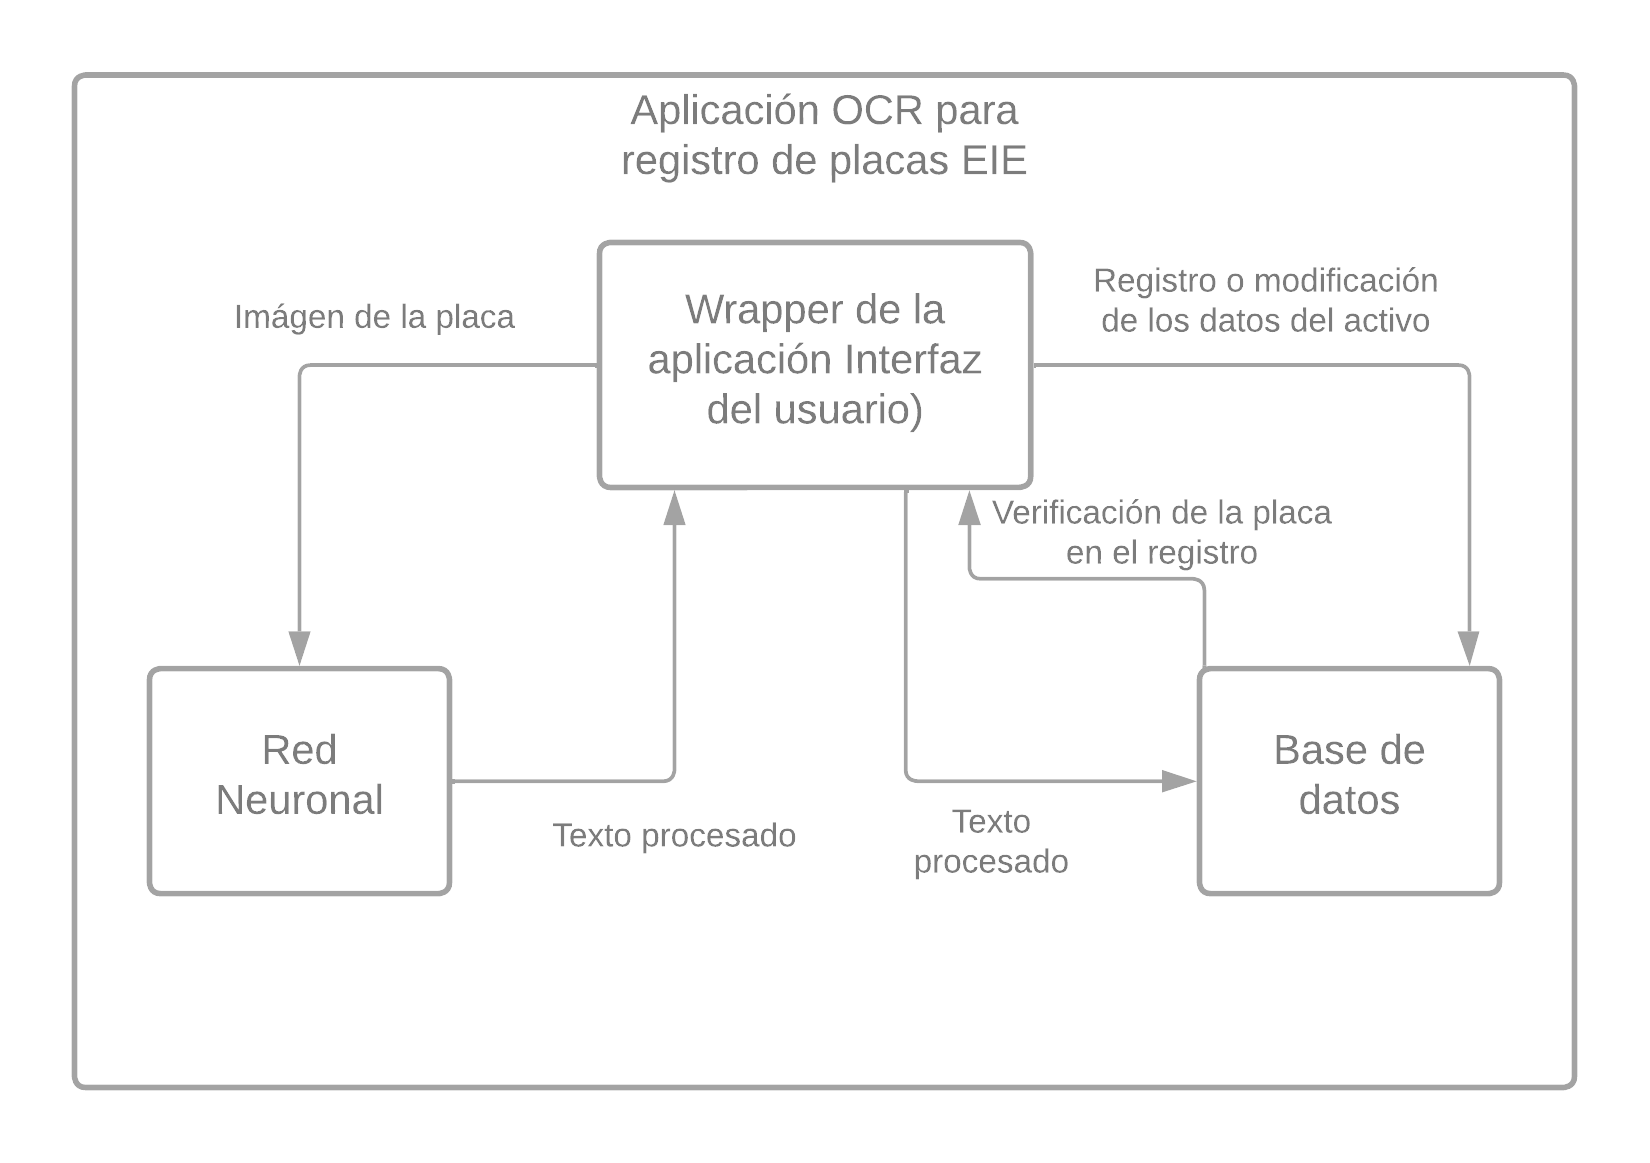
\includegraphics[width=0.7\textwidth]{imagenes/diseño/diagrama_del_programa.png}
    \caption{Diagrama del funcionamiento de la aplicación (creación propia)}
    \label{appdiagram}
\end{figure}
\par
Se crea tres componentes principales para la aplicación, donde el principal sería el wrapper. Sus otros dos componentes son la base de datos, que servirá para almacenar todos los activos con sus respectivos parámetros y la red neuronal, que procesa el texto de las imágenes y entrega el número de placa encontrado en el mismo. Estos se encuentran conectados entre sí por medio del wrapper, que no solamente permite las entradas y las salidas con los usuarios, sino que también corre las funciones para acceder a cada uno de los componentes.

\section{Red neuronal}
Debido a la complejidad y cantidad de recursos que puede requerir crear una red neuronal completamente de cero, se optó por utilizar una basada en la red, a la cual se le modificó diferentes parámetros para procesar específicamente imágenes y que realizaran un análisis de OCR. 
\par
El servicio utilizado para este proyecto fue el de Nanonets, debido a que las redes neuronales que ofrecen permiten nativamente adaptarlas para el reconocimiento y procesamiento de caracteres. Específicamente se consideró el pre-procesamiento de las imágenes y el procesado como los más significativos a la hora de alterar las especificaciones buscadas dentro de lo que iba a analizar la red.
\par
Primeramente se escogió un modelo sin plantilla, es decir su funcionalidad y parámetros se definen desde cero, por lo que se ajustó para que fuese especializada en OCR. Luego se modificó el tipo de preprocesado que reciben las imágenes una vez que son recibidas por el servidor, de la misma forma se incluye dentro de los ajustes de la red escogida. El primer parámetro a corregir es la normalización de la imagen, la cual sirve para cambiar la intensidad de los pixeles a uno adecuado. Luego la corrección de torcimiento (Skew correction), que en caso de que la imagen recibida esté torcida permita verla con un mejor ángulo. Se aplica una reducción de ruido, que realiza un barrido para aclarar la imagen. Por último se tomó en cuenta la aplicación de escala de grises y binarización de la imagen para que resalte de forma correcta el texto de las placas.
\par
Es necesario destacar que no fue necesaria la implementación de código para realizar ninguna de las funciones de pre-procesado ni tampoco para los parámetros del procesado de la red. Lo siguiente llevado a cabo fue la definición del tipo de elementos que debería buscar específicamente la red para devolver como respuesta a la salida. Para ello se pusieron parámetros que eliminasen todo tipo de texto y elementos que no correspondieran a un número y que solamente analizara una única línea, debido a que al ser OCR, podría buscar devolver un texto más grande del necesario. Todo esto es necesario debido a que las placas de la Universidad de Costa Rica (figura \ref{ejem_placa}), poseen no solamente el número de activo, sino que también el logo y nombre de la Universidad.
\begin{figure}[h!]
    \centering
    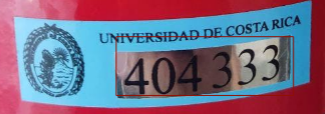
\includegraphics[width=0.5\textwidth]{imagenes/diseño/ejem_placa.PNG}
    \caption{Placa de activo de la Universidad de Costa Rica (ejemplo)}
    \label{ejem_placa}
\end{figure}
\par
La última parte del diseño de la red es el entrenamiento de la misma, por medio de alimentación de datos de entrada. En este caso se utilizó un total de 30 placas capturadas en diferentes activos a través de la facultad de ingeniería y de la EIE. El modelo visto en la Figura \ref{ejem_placa} no es el único existente, sino que se encuentran modelos más antiguos, éstos también fueron considerados dentro del entrenamiento para tener una amplia gama de respuesta por parte de la red. 
\par
Una vez terminado el proceso de entrenamiento se diseñó un código capaz de interactuar con la API de Nanonets, que recibe las imágenes, en este caso en forma de archivo binario, para poder procesarla por medio de la red. La API devuelve una salida con diferentes parámetros escaneados de la imagen en formato JSON, pero únicamente se tomó en cuenta el \lstinline{ocr_text}. La conexión se realizó por medio de el paquete de requests, que permite realizar solicitudes a servidores y servicios API utilizando una llave personal para acceder a ellas (la llave fue provista por Nanonets para la implementación de la aplicación). A continuación se muestran el código de conexión al servidor y para extraer la respuesta respectivamente: 

\begin{lstlisting}[language=Python,frame=single,caption=Código para envío de las placas y recibimiento del texto de la misma (creación propia), inputencoding=latin1]
url = 'https://app.nanonets.com/api/v2/OCR/Model/34353217-1d3f-4511-b86f-e24e842e66e8/LabelFile/?async=false'
data = {'file': open(self.captura_actual, 'rb')}
response = requests.post(url, auth=requests.auth.HTTPBasicAuth('0DeaHQHCf7qAs9n7mFAGmF9gHd6IVMA9', ''), files=data)
\end{lstlisting}

\begin{lstlisting}[language=Python,frame=single,caption=Código para extracción del texto de la placa de la respuesta de la red neuronal (creación propia), inputencoding=latin1]
self.placa_actual = response_json["result"][0]['prediction'][0]['ocr_text']
\end{lstlisting}

\section{Base de datos}
La base de datos se diseñó pensando en que se debía tener un modelo intuitivo que fuese fácil de manipular, donde los datos pudiesen ser exportados de manera sencilla a algún formato conocido por los usuarios. Por ello se utilizó una base de datos relacional, que constará de únicamente una tabla, la cual está definida como la tabla \ref{table1}. 
\begin{table}[h!]
\centering
\resizebox{\columnwidth}{!}{\begin{tabular}{cccc}
\hline
Placa (primary key)        & ubicación                    & tipo de activo           & descripción                              \\ \hline
Número de placa del activo & Donde se encuentra el activo & Clasificación del activo & Descripción más detallada de los activos \\ \hline
\end{tabular}}
\caption{Tabla que se implementó en la base de datos}
\label{table1}
\end{table}

\par
Para la creación de la tabla se instaló un servidor local por medio de la herramienta MySQL, que permitió realizar la base de datos de manera local, para realizar las pruebas necesarias dentro del desarrollo de la aplicación. La creación de la tabla dentro de la base de datos se realizó por medio de un script de Python que accediera a la base de datos y generara una solicitud para una tabla nueva con las columnas definidas previamente. El script además dentro de la creación de las columnas define el \textit{Primary Key}, que representa la identificación de cada uno de los registros, no es necesario hacer una asignación automática, puesto que se utilizaría la placa como identificación de cada uno de los registros. El paquete de python utilizado para la gestión de bases de datos fue el nativo de MySQL llamado MySQL Connector, este se instaló dentro del paquete de MYSQL community. El código del script de Python implementado se puede ver a continuación:
\newpage
\begin{lstlisting}[language=Python,frame=single,caption= Script de python para la conexión a una base de datos (creación propia), inputencoding=latin1]
import mysql.connector

db = mysql.connector.connect(
    host='localhost',
    user='root',
    passwd='InventarioEIE2409',
    database='inventarioeie'
)
mycursor = db.cursor()
\end{lstlisting}
\par
Esta sección de código realiza una conexión simple al servidor local de la base de datos, con los credenciales del usuario root para poder tener manejo completo de la misma. Se definió la base de datos como local, debido a que la implementación no llevó a cabo una implementación en servidor externo para la realización del desarrollo sin embargo, a la hora de lanzar la aplicación para dispositivos móviles, la base de datos se migra y se establecen conexiones directamente con el servidor. Dentro de los accesos realizados más adelante no es necesario utilizar una acceso root, puesto que no se estará modificando la tabla y su estructura, sino únicamente añadiendo y modificando datos dentro. Además crea un cursor, el cual es el encargado de realizar todas las operaciones para la creación de bases de datos, tablas y toda la inserción, eliminación y modificación de datos en general, es decir maneja cada una de las solicitudes a la BD. 
\begin{lstlisting}[language=Python,frame=single,caption= Script de python para la creación de una tabla en una base de datos (creación propia), inputencoding=latin1]
mycursor.execute("CREATE TABLE Activos (placa int PRIMARY KEY, ubicacion TEXT(65535), tipo_de_activo TEXT(65535), descripcion TEXT(65535))")
\end{lstlisting}
\par
La anterior sección del script, únicamente creó la tabla nueva llamada \textbf{Activos}, con todos los parámetros necesarios, definiendo así donde se almacenarían los datos a futuro. Los valores que se dieron al tipo de variable de cada una de las columnas es la longitud que puede tener la misma. Para asegurar una generalidad y funcionamiento seguro, se utilizó el valor máximo para cada tipo de variable (65535 caracteres).
\par
Todas y cada una de las funciones que gestionan los accesos y las escrituras a la base de datos se implementaron como funciones dentro del wrapper de la aplicación, ya que es necesario que el funcionamiento se de durante el uso de la aplicación. 


\section{Wrapper de la aplicación}
 El wrapper de la aplicación tiene como funcionamiento crear una capa que permita la conexión de la base de datos y de la red neuronal con el usuario y entre sí. Se utilizó la biblioteca KivyMD, las cual sirve para la creación de interfaces gráficas multiplataforma. Esto permite que el diseño sea utilizable tanto en la plataforma de desarrollo (donde se usó windows), cómo en la plataforma de distribución (android), ya que los elementos que contiene se adaptan a respuestas físicas (como la de un mouse) y a respuestas táctiles (como en dispositivos móviles).
 \par
 KivyMD es una derivación de la biblioteca Kivy, pero que utiliza un diseño moderno (basado en el estilo gráfico de Android actual Material Design 3) para sus elementos. Se realizó de esta forma para que la experiencia de usuario fuese la mejor posible. 
\par
 Inicialmente se construyó el esqueleto de la aplicación, el cual no contiene elementos en él, pero permite inicializar el funcionamiento. KivyMD utiliza programación orientada a objetos para definir a los esqueletos, por lo que se creó la clase \textbf{Inventario}. Esta clase consta de 8 métodos o funciones internas y un constructor, es posible ver la construcción en la figura \ref{skeleton}.
 \begin{figure}[h!]
    \centering
    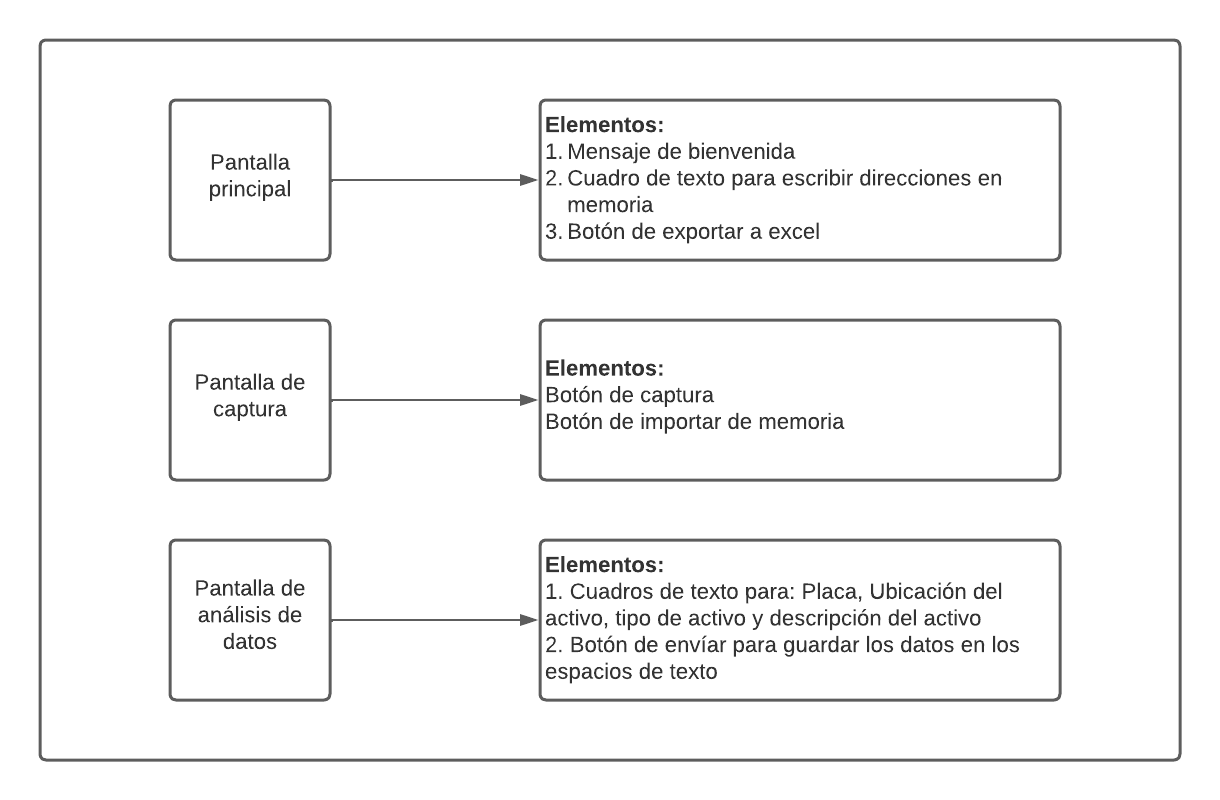
\includegraphics[width=0.7\textwidth]{imagenes/diseño/diagrama_esqueleto.png}
    \caption{Diagrama de bloques del esqueleto de la aplicación}
    \label{skeleton}
\end{figure}
 \par
 El constructor se diseñó con diferentes atributos, los obligatorios establecidos por KivyMD, que son: la versión de Material Design que se utilizó (Material Desing 3) y el tema que utiliza la aplicación (esquema de colores). Luego se definió los atributos propios los cuales fueron: La captura actual (string con la dirección de la captura actual), placa actual (string con la placa que se escaneó más recientemente), \textit{is registered} (booleano que determina si la placa que se escaneó se encuentra previamente almacenada en la base de datos) y por último file manager (permite importar el módulo de file manager de kivyMD para importar archivos directamente de la memoria). El objetivo principal de estas definiciones se basó en la captura de variables de interés que deriven de los métodos de la aplicación.
 \par
 Lo último contenido dentro del constructor, es la pantalla, que importa toda la definición de la interfaz gráfica para mostrarla al usuario. Se escribió las definiciones de la pantalla en la variable \textit{layouts} como un string en lenguaje declarativo de Kivy, que es una forma alternativa, intuitiva y mayormente documentada para el acomodo de los elementos gráficos de la aplicación. En la figura \ref{screen1} se muestra la pantalla principal de la aplicación.
\begin{figure}[h!]
    \centering
    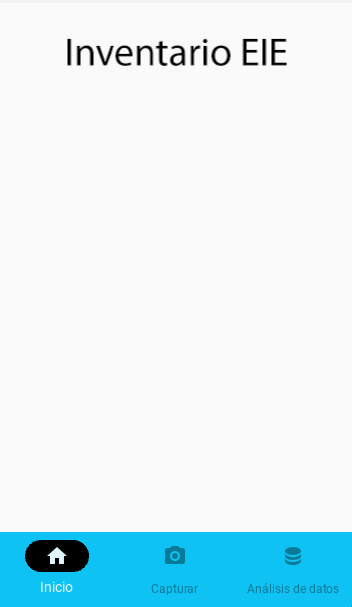
\includegraphics[width=0.35\textwidth]{imagenes/diseño/pantalla1.png}
    \caption{Pantalla principal de la aplicación}
    \label{screen1}
\end{figure}
\par
La forma en la que el lenguaje declarativo de kivy acomoda los elementos de la aplicación es jerárquica, por lo que inicialmente se debió seleccionar el tipo de pantalla deseada, esta usualmente determina como se ve la interfaz general de la aplicación. El nivel principal de la jerarquía que se implementó fue \textit{BottomNavigationLayout}, que contiene una barra inferior con botones para seleccionar la pantalla a la que se accede. Luego en nivel 2 se definió 3 pantallas: inicio, captura y análisis de datos. El nivel 3 siendo el último nivel contiene los elementos dentro de las 3 pantallas del nivel 2.
\par
La pantalla de inicio o pantalla principal, despliega el logo de la aplicación, que se creó a partir de la tipografía de la EIE, un mensaje de bienvenida para los usuarios, un cuadro de texto para que los usuarios indiquen una dirección en la memoria (en este caso de la computadora, debido a que la implementación en Android quedó fuera del diseño para éste proyecto) y un botón que activa la función \verb|import_to_excel(self)|.
\par
La función \verb|import_to_excel(self)|, implementa la conexión a la base de datos definida anteriormente y por medio del cursor importa todos los datos de la tabla de activos. Una vez importados los datos, con la ayuda de la biblioteca pandas se convierte a un marco de datos, que puede ser exportado a Excel por una función de pandas, la exporrtación se realiza en la dirección especificada por el usuario en un archivo llamado \textbf{activos.xlsx}. 
\begin{figure}[h!]
    \centering
    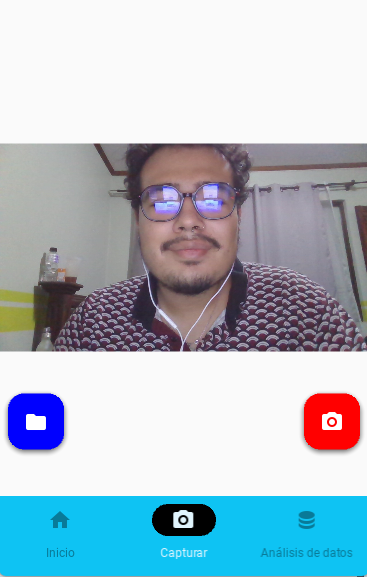
\includegraphics[width=0.35\textwidth]{imagenes/diseño/pantalla2.png}
    \caption{Pantalla de captura de la aplicación}
    \label{screen2}
\end{figure}
\par
La pantalla de captura, que se mostró en la figura \ref{screen2}, contiene 3 elementos: Una imagen en tiempo real de la cámara principal del dispositivo que corre la aplicación, un botón de captura y un botón de carga de archivos. El botón de captura al ser presionado activa la función \verb|capture(self)|, que almacena en la ubicación actual la imagen de la cámara, asignando un nombre con único y aleatorio, guarda la dirección completa del archivo en \verb|self.captura_actual| y activa la función de \verb|ocr_scan(self)|. 
\par
El botón de carga al ser presionado activa la función \verb|open_manager(self)|, que abre un explorador de archivos (implementado por KivyMD) en el disco duro principal del dispositivo, como se muestra en la figura \ref{xplorer} y una vez se selecciona el archivo deseado, se asigna la ruta a \verb|self.captura_actual| por medio de la función \verb|select_path(self, path: str)| y el algoritmo procede de la misma forma que con el botón de captura. Internamente cuando se selecciona el archivo o se cierra el explorador la función \verb|exit_manager(self, *args)| finaliza la instancia que lo trajo a pantalla.
\par
\begin{figure}[h!]
    \centering
    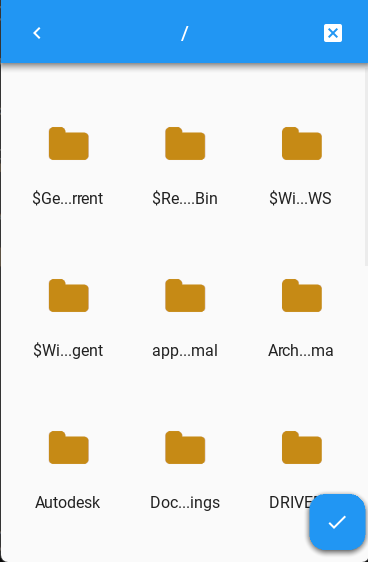
\includegraphics[width=0.35\textwidth]{imagenes/diseño/explorador.png}
    \caption{Explorador de archivos}
    \label{xplorer}
\end{figure}
En caso de que la imagen se procesó correctamente en \verb|ocr_scan(self)|, se muestra un mensaje en pantalla para que el usuario avance al análisis de datos y contrariamente un mensaje de error para que el usuario vuelva a tomar o importar la foto.
\par
La función \verb|ocr_scan(self)| implementa tanto el Listing 3.1 cómo el Listing 3.2, si el API de Nanonets devuelve una respuesta con la placa procesada en formato de string retorna un \verb|True|, de lo contrario un \verb|False|, que sirve para activar los mensajes finales en la función de captura.
\par
\begin{figure}[h!]
    \centering
    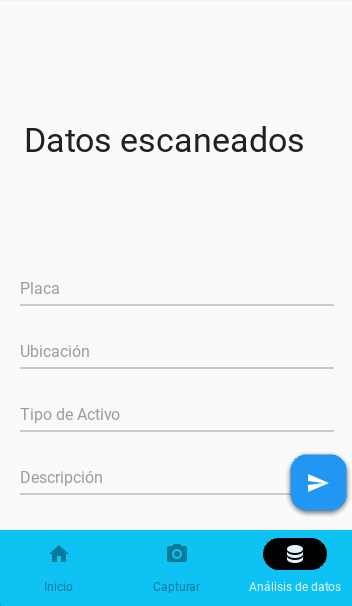
\includegraphics[width=0.30\textwidth]{imagenes/diseño/pantalla3.png}
    \caption{Pantalla de análisis de datos de la aplicación}
    \label{screen3}
\end{figure}
Por último la pantalla de análisis de datos, mostrada en la figura \ref{screen3}, inicialmente al ser presionada activa la función \verb|rev_placa(self)| que se diseñó para verificar la existencia de la placa escaneada dentro de la base de datos. La función inicialmente conecta con el servidor, crea un cursor para ejecutar solicitudes para luego importar todos los datos de la BD. Antes de buscar la placa actual entre todos los datos registrados, pone el valor de \verb|self.is_registered| en falso y si la función logra encontrarla dentro dde la DB, la convierte en verdadero. Cuando \verb|self.is_registered| se encuentra en verdadero, despliega un mensaje en pantalla avisando al usuario de la existencia previa y de la posibilidad de modificar los valores directamente en los campos de texto. Si \verb|self.is_registered| está en falso, se sustituye únicamente el valor de la placa y se despliega un aviso para que el usuario proceda a llenar los datos del activo.
\par
Cuando el usuario decide que ya modificó o agregó los datos del registro, únicamente debe tocar el botón de envío, que activa la función \verb|registrar_placa(self)|. Inicialmente la función conecta con el servidor y crea un cursor, para de forma seguida analizar \verb|self.is_registered|, debido a que los procesos de un registro nuevo y la modificación de un registro son distintos. Cuando el atributo es verdadero se utilizó el siguiente código:

\begin{lstlisting}[language=Python,frame=single,caption= Modificación de registro previamente existente (creación propia), inputencoding=latin1]
mycursor.execute("UPDATE Activos SET ubicacion = %s, tipo_de_activo = %s, descripcion = %s WHERE placa = %s", (self.root.ids.ubicacion.text, self.root.ids.active_type.text, self.root.ids.descrip.text, self.placa_actual))
            db.commit()
            toast("Placa actualizada!")
\end{lstlisting}
\par
Los parámetros dentro del \verb|execute|, corresponden a los strings contenidos en las cajas de texto de la pantalla de análisis de datos. Cuando no se encuentra el valor registrado en la BD, el código que se usó fue el siguiente:

\begin{lstlisting}[language=Python,frame=single,caption= Registro nuevo de activo (creación propia), inputencoding=latin1]
mycursor.execute("INSERT INTO Activos (placa, ubicacion, tipo_de_activo, descripcion) VALUES (%s, %s, %s, %s)", (self.placa_actual, self.root.ids.ubicacion.text, self.root.ids.active_type.text, self.root.ids.descrip.text))
            db.commit()
            toast("Placa registrada!")
\end{lstlisting}
\par
De esta forma se definió el wrapper y sus elementos, que implementan los otro módulos del diseño inicial, afirmando así la base que se mostró en la figura \ref{appdiagram}. 






